\section{Modi di indirizzamento}
Ci sono diversi modi per prendere i dati da utilizzare nei calcoli.

\subsection{Indirizzamenti}

\subsubsection{Indirizzamento a registro}
Se il dato si trova all'interno di un registro ci basterà specificare il nome del registro per poterlo utilizzare:
\begin{verbatim}
    ADD r7, r9 # r7 <- r7 + r9
\end{verbatim}

\subsubsection{Indirizzamento immediato}
Se il dato è disponibile a tempo di compilazione possiamo inserirlo direttamente nella istruzione.
Possiamo specificarlo solamente come operando sorgente, ovviamente.
Per indicare questo indirizzamento si aggiunge una "I" alla fine dell'istruzione:
\begin{verbatim}
    ANDI r17, 0x41 # r17 <- r17 AND 0x41
\end{verbatim}

I valori possono essere specificati in:
\begin{itemize}
    \item decimale, con e senza segno:
    \begin{verbatim}
        SUBI r17, 13
        SUBI r17, -13
    \end{verbatim}
    
    \item esadecimale, preceduto da "0x":
    \begin{verbatim}
        SUBI r17, 0xD
    \end{verbatim}
    
    \item binario, preceduto da "0b":
    \begin{verbatim}
        SUBI r17, 0b00001101
    \end{verbatim}
    
    \item espressioni da calcolare: solo se le espressioni sono calcolabili a tempo di assemblaggio
    \begin{verbatim}
        LDI r18, 5*3
        LDS r9, 0x0870 + 5
    \end{verbatim}
\end{itemize}


NB: le istruzioni ADDI e ADCI non esistono, bisogna ricorrere a SUBI e SBCI e cambiare di segno l'operando immediato.

\subsubsection{Indirizzamento diretto}
Questa architettura, essendo RISC, non supporta operazioni memoria-registro o registro-memoria, bisogna utilizzare una istruzione per caricare il valore all' interno di un registro e successivamente usare il registro per fare i calcoli.
\begin{verbatim}
    LDS r9, 0x0870  # legge il byte nella SRAM all'indirizzo 
                    # 0x0870 e ricopia in r9
                    
    STS 0x0870, r9  # scrive il byte contenuto in r9
                    # all'indirizzo 0x0870 della SRAM
\end{verbatim}

\begin{figure}[H]
    \centering
    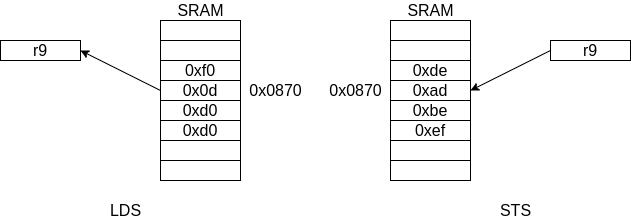
\includegraphics[width=300px]{images/5_Indirizzamento/LDS_STS.png}
\end{figure}

\subsubsection{Indirizzamento diretto con registro puntatore}
Esistono degli alias per alcune coppie di registri:
\begin{itemize}
    \item r31:r30 è identificato da Z
    \item r29:r28 è identificato da Y
    \item r27:r26 è identificato da X
\end{itemize}
queste coppie, e le relative label, sono usati per inserire degli indirizzi da usare per eseguire letture in memoria:
\begin{verbatim}
    LD r9, X  # legge dalla memoria all'indirizzo
              # contenuto in X
\end{verbatim}
Per inserire l'indirizzo nel registro X possiamo usare due modi:
\begin{verbatim}
    LDI r26, 0x70
    LDI r27, 0x08
        # utilizzando r27, r26
    
    LDI XL, 0x70
    LDI XH, 0x08
        # utilizzando gli alias
\end{verbatim}

Per accessi più complessi possiamo utilizzare alcuni operatori sui registri X, Y, Z:
\begin{verbatim}
    LD r10, X+  # legge da X ed incrementa X
            X-  # legge da X e decrementa X
            +X  # incrementa X e poi legge da X
            -X  # decrementa X e poi legge da X
\end{verbatim}

NB: non tutti e 3 i registri implementano tutte e 4 le modalità, il set di istruzioni \emph{non è ortogonale}!

Con il registro Y esiste anche:
\begin{verbatim}
    LD r11, Y + 4
        # legge all'indirizzo Y + 4
        # NON altera il contenuto di Y!
        # l'offset non può essere più grande di 6 bit
        # si possono usare negativi
\end{verbatim}



